\chapter{Data Tools}


\section{Basic Statistics}
You live near a freeway, and someone asks you, ``How fast do cars on that freeway drive?''

You say, ``Pretty fast.''

They reply, ``Can you be more specific?''

So, you pull out your radar gun you happen to always keep on you, and tell them, ``That one is going 32.131 meters per second.''

To which they say, ``I do not want to know about that specific car. I want to know about all the cars.''

So, you spend the day beside the freeway measuring the speed of every
car that goes by. And you get a list of a thousand numbers, including:

\begin{tabular}{c | c | c}
30.462 m/s  & 29.550 m/s & 29.227 m/s \\
37.661 m/s  & 27.899 m/s & 28.113 m/s \\
24.382 m/s & 35.668 m/s & 43.797 m/s \\
31.312 m/s & 37.637 m/s & 30.891 m/s
\end {tabular}

There are 12 numbers here. We say that there are 12 \textit{samples}.\index{samples}

\subsection{Mean}
\textbf{Worked example: the mean of five scores.} A teacher records the scores 62, 70, 70, 85, and 91. The sum is $62 + 70 + 70 + 85 + 91 = 378$. Divide by the number of scores, $n = 5$: the mean is $\bar{x} = \frac{378}{5} = 75.6$.


We often talk about the \textit{average} of a set of samples, which is the 
same as the \textit{mean}. To get the mean, sum up the
samples and divide that number by the number of samples.\index{mean}

The numbers in that table sum to $388.599$.  If you divide that by 12,
you find that the mean of those samples is 32.217 m/s.

We typically use the greek letter $\mu$ (``mu'') to represent the mean.

\begin{mdframed}[style=important, frametitle={Definition of Mean}]
  
If you have a set of samples $x_1, x_2, \ldots, x_n$, the mean is:

$$ \mu = \frac{1}{n} \sum_{i=1}^n x_i$$

\end{mdframed}

This may be the first time you are seeing a summation ($\sum$). The equation above is equivalent to:\index{summation symbol}

$$ \mu = \frac{1}{n} \left(x_1 + x_2 + \ldots + x_n\right)$$

\begin{Exercise}[title={Mean Grade}, label=grades_mean]

  Teachers often use the mean for grading. For example, if you took
  six quizzes in a class, your final grade might be the mean of the six
  scores. Find the mean of these six grades: 87, 91, 98, 65, 87, 100.

\end{Exercise}
\begin{Answer}[ref=grades_mean]

  $$\mu =\frac{1}{6} \left(87 + 91 + 98 + 65 + 87 + 100 \right) = 88$$

\end{Answer}

If you tell your friend, ``I measured the speed of 1000 cars, and the
mean is 31.71 m/s'', your friend will wonder, ``Are most of the speeds
clustered around 31.71? Or are they all over the place and just happen
to have a mean of 31.71?'' To answer this question, we use variance.

\subsection{Variance}

\begin{mdframed}[style=important, frametitle={Definition of Variance}]

If you have $n$ samples $x_1, x_2, \ldots, x_n$ that have a mean of $\mu$, the \textit{variance} is defined to be:\index{variance}

$$v = \frac{1}{n}\sum_{i = 1}^{n} \left(x_i - \mu\right)^2$$
% ADD: Maybe connect to Chi-squared test
\end{mdframed}

That is, you figure out how far each sample is from the median, you
square that, and then you take the mean of all those squared
distances.

\begin{tabular} {c | c | c}

  $x$ & $x - \mu$ & $(x - \mu)^2$\\
  \hline
30.462 & -1.755 & 3.079 \\
29.550 & -2.667 & 7.111\\
29.227 & -2.990 & 8.938\\
37.661 & 5.444 & 29.642\\
27.899 & -4.318 & 18.642\\
28.113 & -4.104 & 16.839 \\
24.382 & -7.835 & 61.381 \\
35.668 & 3.451 & 11.912 \\
43.797 & 11.580 & 134.106\\
31.312 & -0.905 & 0.818\\
37.637 & 5.420 & 29.381\\
30.891 & -1.326 & 1.757\\
\hline
$\sum x = 386.599$ & & $\sum (x - \mu)^2 = 323.605$\\
mean = 32.217 & & variance = 26.967
\end{tabular}

Thus, the variance of the 12 samples is 26.967. The bigger the variances, 
the farther the samples are spread apart; the smaller the variances, the closer
samples are clustered around the mean.

Notice that most of the data points deviate from the mu by 1 to 5
m/s. Is not it odd that the variance is a big number like 26.967?
Remember that it represents the average of the squares. Sometimes, to
get a better feel for how far the samples are from the mean, we use
the square root of the variance, which is called \textit{the standard
  deviation}.

The \index{standard deviation}standard deviation of your 12 samples would be $\sqrt{26.9677} =
  5.193$ m/s.
% ADD: Bell curve, KA: https://www.khanacademy.org/computer-programming/spin-off-of-galton-board-exploration/1930953307/embedded?embed=yes&article=yes&editor=no&buttons=no&author=no&width=400&height=400

The standard deviation is used to figure out if a data point is an
\index{outlier}outlier. For example, if you are asked, ``That car that just sped
past. Was it going freakishly fast?'' You might respond, ``No, it was
within a standard deviation of the mean.'' or ``Yes, its speed was 2
standard deviations more than the mean. They will probably get a ticket.''
% ADD: Box and whiskers plot?

A singular $\mu$ usually represents the mean. $\sigma$ usually represents
the standard deviation. So $\sigma^2$ represents the variance.

\begin{Exercise}[title={Variance of Grades}, label=grades_variance]

  Now, find the variance for your six grades. As a reminder, they were: 87, 91, 98, 65, 87, 100.

  What is your standard deviation?

\end{Exercise}
\begin{Answer}[ref=grades_variance]

  The mean of your grades is $88$.

  The variance, then, is

  $$\sigma^2 = \frac{1}{6} \left((87 - 88)^2 + (91 - 88)^2 + (98 - 88)^2 + (61 - 88)^2 + (87 - 88)^2 + (100 - 88)^2 \right) = \frac{784}{6} = 65 \frac{1}{3}$$

  The standard deviation is the square root of that: $\sigma = 8.083$ points.
  
\end{Answer}


\subsection{Median}

Sometimes you want to know where the middle is. For example, you want
to know the speed at which half the cars are going faster and half are
going slower. To get the median, you sort your samples from smallest
to largest. If you have an odd number of samples, the one in the
middle is the median. If you have an even number of samples, we take
the mean of the two numbers in the middle.\index{median}
% KA: https://www.khanacademy.org/math/cc-sixth-grade-math/cc-6th-data-statistics/mean-and-median/v/statistics-intro-mean-median-and-mode

In our example, you would sort your numbers and find the two in the middle:

\begin{tabular}{c}
24.382\\
27.899\\
28.113\\
29.227\\
29.550\\
\hline
\textbf{30.462}\\
\textbf{30.891}\\
\hline 
31.312\\
35.668\\
37.637\\
37.661\\
43.797\\
\end{tabular}

You take the mean of the two middle numbers: $(30.462 + 30.891)/2 =
30.692$. The median speed would be 30.692 m/s.

Medians are often used when a small number of outliers majorly skew the
mean. For example, income statistics usually use the median income
because a few hundred billionaires raise the mean a great deal.

\begin{Exercise}[title={Median Grade}, label=grades_median]

  Find the median of your six grades: 87, 91, 98, 65, 87, 100.

\end{Exercise}
\begin{Answer}[ref=grades_median]

  In order the grades are 65, 87, 87, 91, 98, 100.  The middle two are 87
  and 91. The mean of those is 89. (Speed trick: The mean of two numbers is the
  number that is halfway between.)
  
 \end{Answer}


\subsection{Histograms and Bell Curves}

A histogram is a bar chart that shows how many samples are in each
group. In our example, we group cars by speed. Maybe we count the
number of cars going between 30 and 32 m/s. Next, we count the
cars going between 32 and 34 m/s. Finally, we make a bar chart from
that data.\index{histograms}
% ADD: Have not explained histograms yet


Your 1000 cars would break up into these groups:

\begin{tabular}{ c | c }
0 - 2 m/s & 0 cars \\
2 - 4 m/s & 0 cars \\
4 - 6 m/s & 0 cars \\
\ldots & \ldots \\
20 - 22 m/s & 0 cars \\
22 - 24 m/s & 0 cars \\
24 - 26 m/s & 65 cars \\
26 - 28 m/s & 160 cars \\
28 - 30 m/s & 175 cars \\
30 - 32 m/s & 168 cars \\
32 - 34 m/s & 150 cars \\
34 - 36 m/s & 114 cars \\
36 - 38 m/s & 79 cars \\
38 - 40 m/s & 52 cars \\
40 - 42 m/s & 20 cars \\
42 - 44 m/s & 12 cars \\
44 - 46 m/s & 4 cars \\
46 - 48 m/s & 1 cars \\
48 - 50 m/s & 0 cars \\
\end{tabular}

Next, we make a bar chart from that:

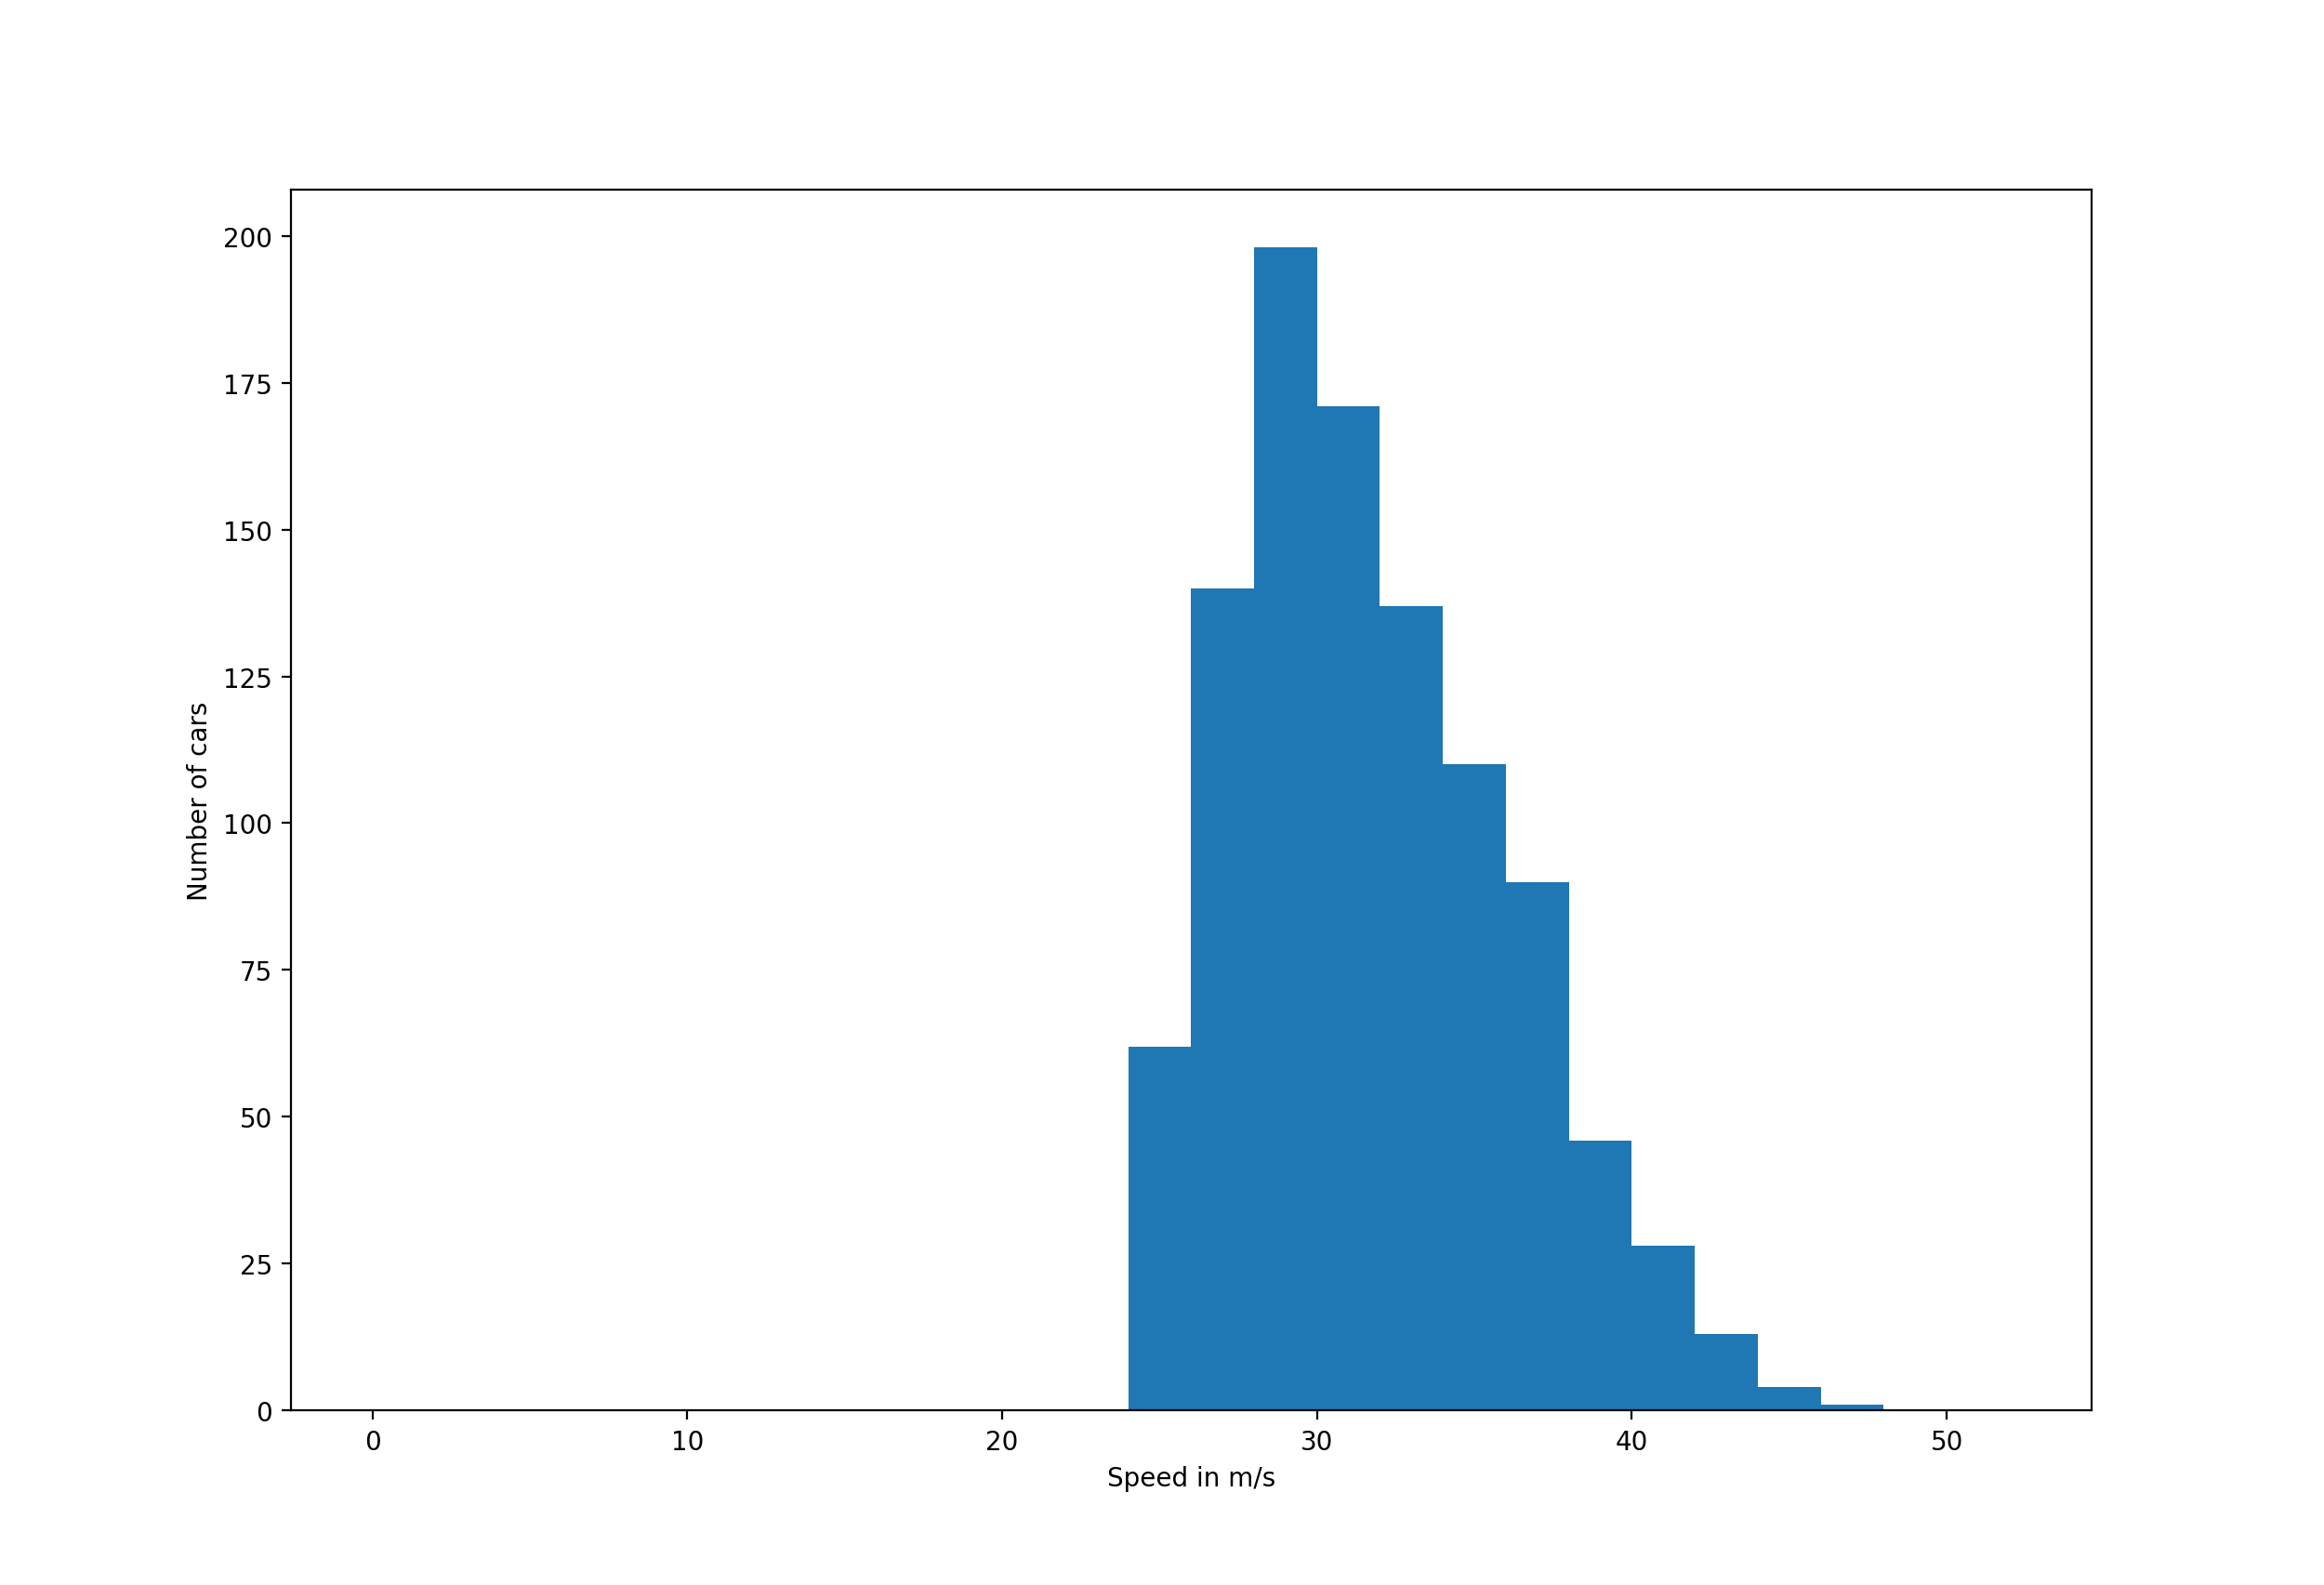
\includegraphics[width=\textwidth] {speed_histo.png}

Often, a histogram will tell the story of the data. Here, you can see
that no one is going less than 24 m/s, but a lot of people travel at
30 m/s. There are a few people who travel over 40 m/s, but there are also a
couple of people who drive much faster than anyone else.
% FIXME added bell curve section - arjan
% may need editing 

If we look closely at the shape of our histogram, we notice something interesting: it has a smooth, rounded hill in the middle and it tapers off on both sides. This is a common pattern in statistics, and it often suggests that the data follows what is called a \textbf{normal distribution}, also known as a \textbf{bell curve}.\index{bell curve}\index{normal distribution}

A \textbf{bell curve} is a continuous curve that models how data is distributed when:
\begin{itemize}
    \item Most values are near the average (mean), located at the peak of the curve,
    \item Fewer values are far from the mean, the tails of the curve,
    \item The distribution is roughly symmetric.
\end{itemize}

In our case, the majority of cars are traveling around 30--32 m/s. There are fewer cars going slower or faster than that. If we collected even more data (say, 10{,}000 cars), the histogram would start to resemble a smooth bell curve even more closely. The units of the x-axis (speed) would still be the same, but the y-axis would represent the \index{probability density}\textit{probability density} of finding a car at a certain speed, rather than just the count of cars in each speed range.

% ADD: image with drawn bell curve around it
%\begin{center}
% FIXME: Commit images.
%\includegraphics[width=0.8\textwidth]{bell_curve_example.png}
%\end{center}

The peak of the bell curve represents the \textbf{mean speed}, and the spread of the curve is related to the \textbf{standard deviation} — a measure of how spread out the speeds are. Most data falls within:
\begin{itemize}
    \item 1 standard deviation of the mean ($\mu \pm \sigma$): about 68\% of the cars,
    \item 2 standard deviations: about 95\%,
    \item 3 standard deviations: about 99.7\%.
\end{itemize}

This means that if we know the mean speed and the standard deviation, we can predict how many cars will be within certain speed ranges. If you have ever heard of \index{Six Sigma}Six Sigma methodology, that means data falls within six standard deviations of the mean, which is a very high level of quality control (3.4 defects per million measurements!).

So when we say a dataset "looks like a bell curve," we mean that it has a predictable and symmetric structure, often meaning it is a reliable set of data with few outliers and consistent results.


\subsection{Root-Mean-Squared}

Scientists have a mean-like statistic that they love. It is named
quadratic mean, but most just calls it Root-Mean-Squared, or
RMS.

\begin{mdframed}[style=important, frametitle={Definition of RMS}]

If you have a list of numbers $x_1, x_2, \ldots, x_n$, their RMS
is \index{quadratic mean} \index{root-mean-squared} \index{RMS}

$$\sqrt{\frac{1}{n}\left( x_1^2 + x_2^2 + \ldots + x_n^2 \right)}$$

\end{mdframed}

You are taking the square root of the mean of squares of the samples,
thus the name Root-Mean-Squared.

Using your 12 samples:

\begin{tabular}{c |  c}
  $x$ & $x^2$ \\
  \hline
30.462 & 927.933 \\
29.550 & 873.203\\
29.227 & 854.218\\
37.661 & 1418.351\\
27.899 & 778.354\\
28.113 & 790.341\\
24.382 & 594.482\\
35.668 & 1272.206\\
43.797 & 1918.177\\
31.312 & 980.441\\
37.637 & 1416.544\\
30.891 & 954.254\\
\hline
\multicolumn{1}{r}{Mean of $x^2$} & {1064.875}\\
\multicolumn{1}{r}{RMS} & {32.632}
  \end{tabular}

Why is RMS useful? Let us say that all cars had the same mass $m$, and
you need to know what the average kinetic energy per car is. If you
know the RMS of the speeds of the cars is $v_{rms}$, the average kinetic energy for
each car is

$$k = \frac{1}{2}m v_{rms}^2$$

(You do not believe me? Let us prove it. Substitute in the RMS:

$$k = \frac{1}{2}m \sqrt{\frac{1}{n}\left( x_1^2 + x_2^2 + \ldots + x_n^2 \right)}^2$$

The square root and the square cancel each other out:

$$k = \frac{1}{2}m \frac{1}{n}\left( x_1^2 + x_2^2 + \ldots + x_n^2 \right)$$

Use the distributive property:

$$k = \frac{1}{n} \left( \frac{1}{2} m x_1^2 + \frac{1}{2}m x_2^2 + \ldots + \frac{1}{2}m x_n^2 \right)$$


That is all the kinetic energy divided by the number of cars, which is
the mean kinetic energy per car. Quod erat demonstrandum! (That is a
Latin phrase that means ``which is what I was trying to
demonstrate''. You will sometimes see ``QED'' at the end of a long
mathematic proof.)

Now you are ready for the punchline: Kinetic energy and heat are the
same thing. Instead of cars, heat is the kinetic energy of molecules
moving around. More on this soon.

Video: Mean, Median, Mode: https://www.youtube.com/watch?v=5C9LBF3b65s


\section{Basic Statistics in Spreadsheets}
When you completed the problems in the last section, you probably noticed
how long it took to compute statistics like the mean, median,
and variance by hand. Luckily, computers were designed to free us from these
sorts of tedious tasks. The most basic tool for automating
calculations is the spreadsheet program.\index{spreadsheet}

The first spreadsheet program (VisiCalc) was introduced in 1979 as a
tool for finance people to play ``what if'' games.  For example, a
company might make a spreadsheet that told them how much more profit
they would make if they changed from using an expensive metal to using
a cheaper alloy.

There are lots of spreadsheet programs, including Microsoft's Excel, Google Sheets, and
Apple's Numbers. Any spreadsheet program will work; they are all very
similar. The instructions and screenshots here will be from Google
Sheets --- a free spreadsheet program you use through your web browser.

\subsection{The Barrel Problem}
In honor of this history, let us start by studying a business question:
You have a friend who dreams of quitting her job to become a cooper. (A
cooper makes barrels that are used for aging wine and whiskey.)  According to her:
\begin{itemize}
\item It costs \$45 dollars in materials to build one barrel.
\item A barrel sells for \$100 dollars.
\item The workshop/warehouse she wants to rent costs \$2000 per month.
\item Taxes take 20\% of her profits.
\item She needs to make \$4000 monthly after taxes.
\end{itemize}

She has asked you, ``How many barrels do I need to make each month?''


\subsection{Solving It Symbolically}

Many problems can be solved two ways: symbolically or
numerically.\index{symbolic vs. numeric solutions} To solve this
problem symbolically, you would write out the facts as equations or
inequalities, then do symbol manipulations until you ended up with
an answer. In this case, you would let $b$ be the number of barrels
and create the following inequality:

$$(1.0 - 0.2)\left(b(100 - 45) - 2000\right) \geq 4000$$

You would simplify it:

$$(0.8)\left(55 b - 2000\right) \geq 4000$$

And simplify it more:

$$44b - 1600 \geq 4000$$

If that is true, then:

$$44b \geq 5600$$

And if that is true, then:

$$b \geq \frac{1400}{11}$$

$1400/11$ is about 127.27, so she needs to make and sell 128 barrels
each month.

That is a perfect answer, and we did not need a spreadsheet at all. However:
\begin{itemize}
\item As problems get larger and more realistic, it gets much more difficult to solve them symbolically.
\item As soon as you say ``Yes, you need to make and sell 128 barrels
  each month.'' Your friend will ask ``What if I make and sell 200
  barrels? How much money will I make then?''
\end{itemize}

So, we use a spreadsheets to solve the problem numerically.


\subsection{Your First Spreadsheet}

Let us first make an initial spreadsheet. 

In whatever spreadsheet program you are using, create a new spreadsheet document.

A spreadsheet is essentially a grid of cells. In each cell, you can put data (like numbers or text) and formulas.

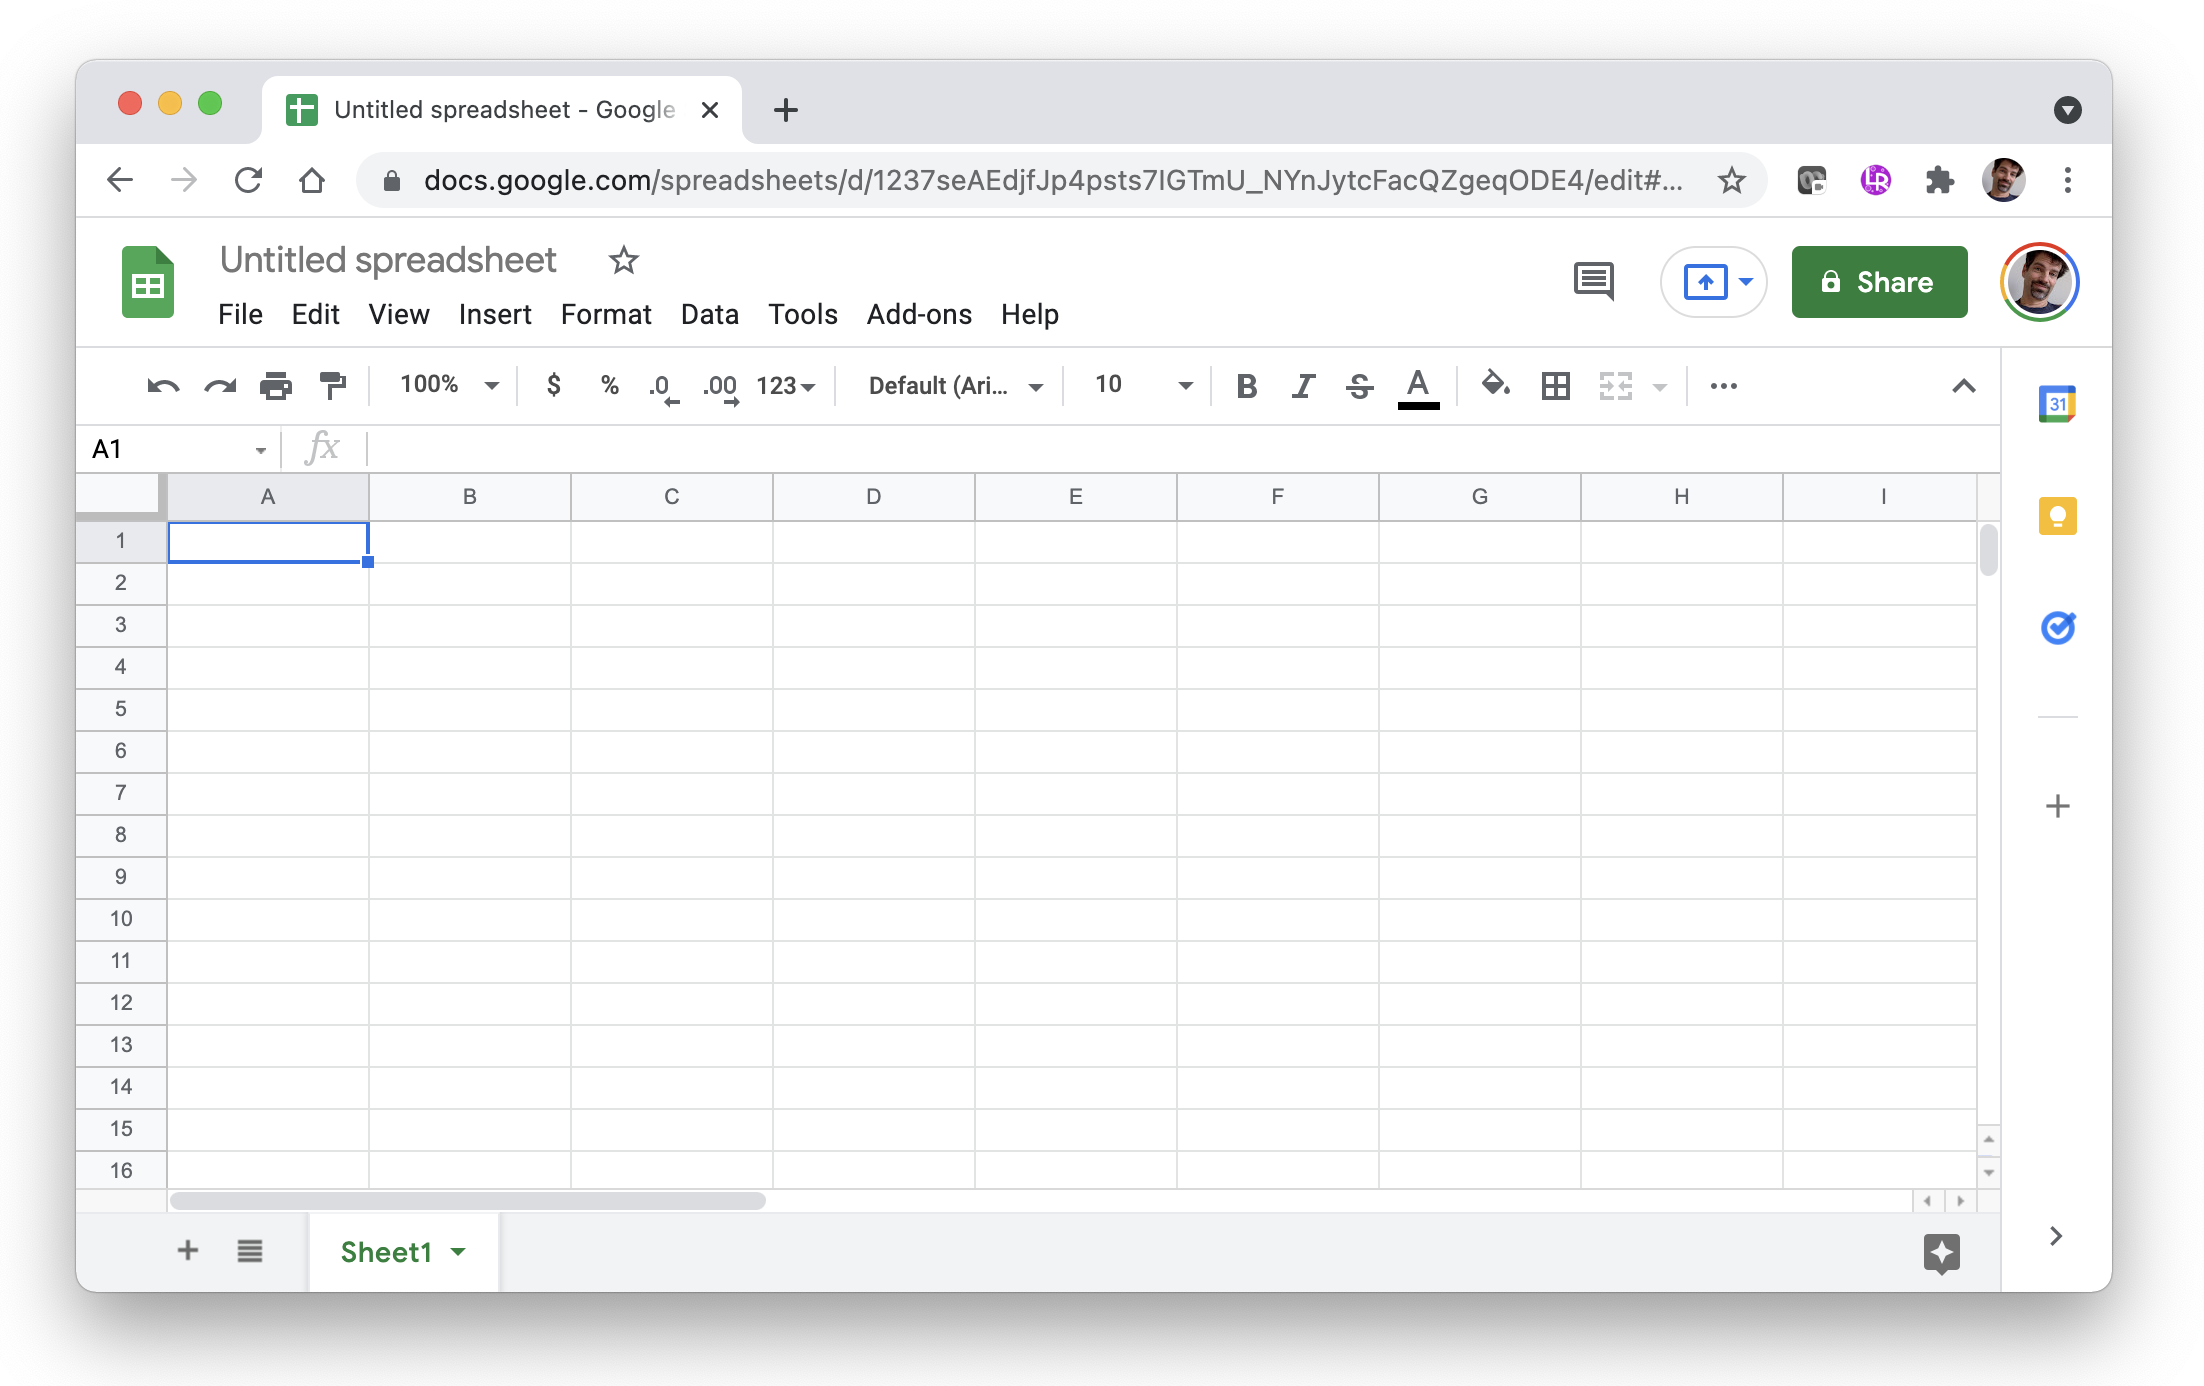
\includegraphics[width=0.6\textwidth]{BlankSheet.png}

Let us put some labels in the column:
\begin{itemize}
\item Select the first cell (A1) and type ``A number''.
\item Select the cell below it (A2) and type ``Another number''.
\item Select the cell below that one (A3) and type ``Their product''.
\item In the next column, type the number 5 in B1 and 7 in B2.
\end{itemize}

It should look like this:

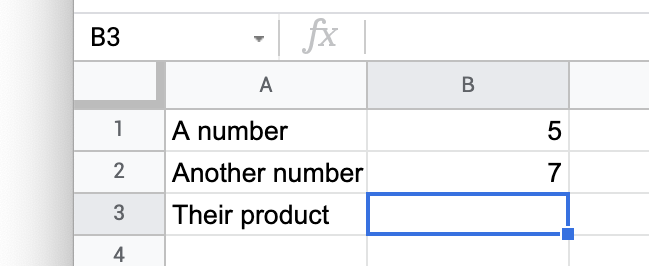
\includegraphics[width=0.5\textwidth]{NoFormulas.png}

Now, put a formula in cell B3. Select B3, and type ``= B1 * B2''. The spreadsheet knows this is a formula because it starts with `=`. It will look like this as you type:\index{Spreadsheet!Entering formula}

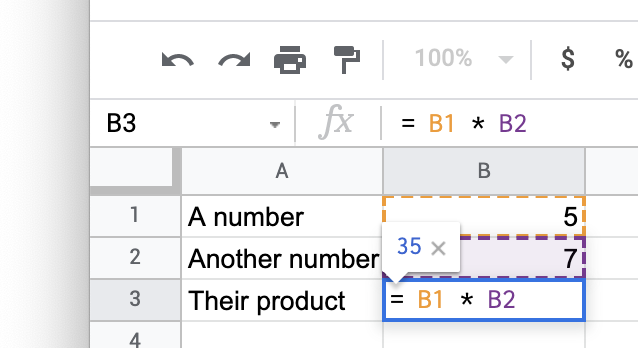
\includegraphics[width=0.5\textwidth]{TypingFirstFormula.png}

When you press Return or Tab, the spreadsheet will remember the formula, but display its value:

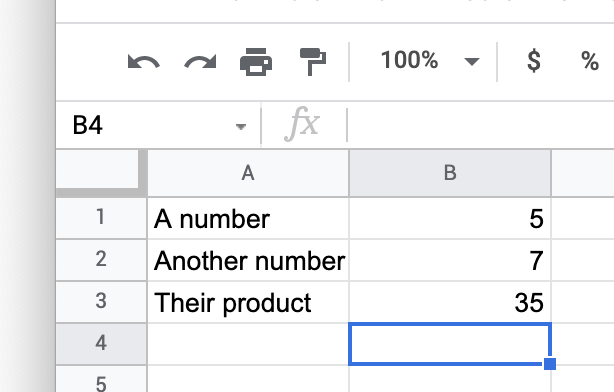
\includegraphics[width=0.5\textwidth]{FirstCalc.png}

If you change the values of cell B1 or B2, the cell B3 will automatically be recalculated. Try it.

\subsection{Formatting}

Every spreadsheet lets you change the formatting of your columns and cells. They are all a little different, so play with your spreadsheet a little now. Try to do the following:
\begin{itemize}
\item Set the background of the first column to light gray.
\item Right-justify the text in the first column.
\item Make the text in the first column bold.
\item Make the numbers in the second column have one digit after the decimal point.
\end{itemize}

It should look something like this:

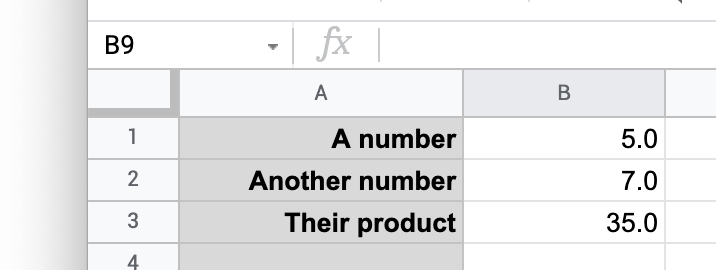
\includegraphics[width=0.6\textwidth]{FirstFormatting.png}

That is a spreadsheet. You have a grid of cells, each of which can hold a
value or a formula that uses values from other cells. The cells containing
formulas automatically update as you edit the values in the other
cells.

\subsection{Comma-Separated Values}

A large amount of data is exchanged in a file format called
\textit{Comma-Separated Values}\index{comma-separated values} or just CSV. Each CSV file holds one
table of data. It is a text file, and each line of text corresponds to
one row of data in the table. The data in each column is separated by
a comma. The first line of a CSV is usually the names of the
columns. A CSV might look like this:

\begin{minted}{python}
studentID,firstName,lastName,height,weight
1,Marvin,Sumner,260,45.3
2,Lucy,Harris,242,42.2
3,James,Boyd,261,44.2
\end{minted}

In your digital resources for this module, you should have a file
called \path{1000cars.csv}. It is a CSV with only one column called
``speed''. The first few lines look like this:

\begin{minted}{python}
speed
33.8000
29.9920
34.8699
27.9936
\end{minted}

There is a title line and 1000 data lines.

Import this CSV into your spreadsheet program. In Google Sheets, it looks like this:

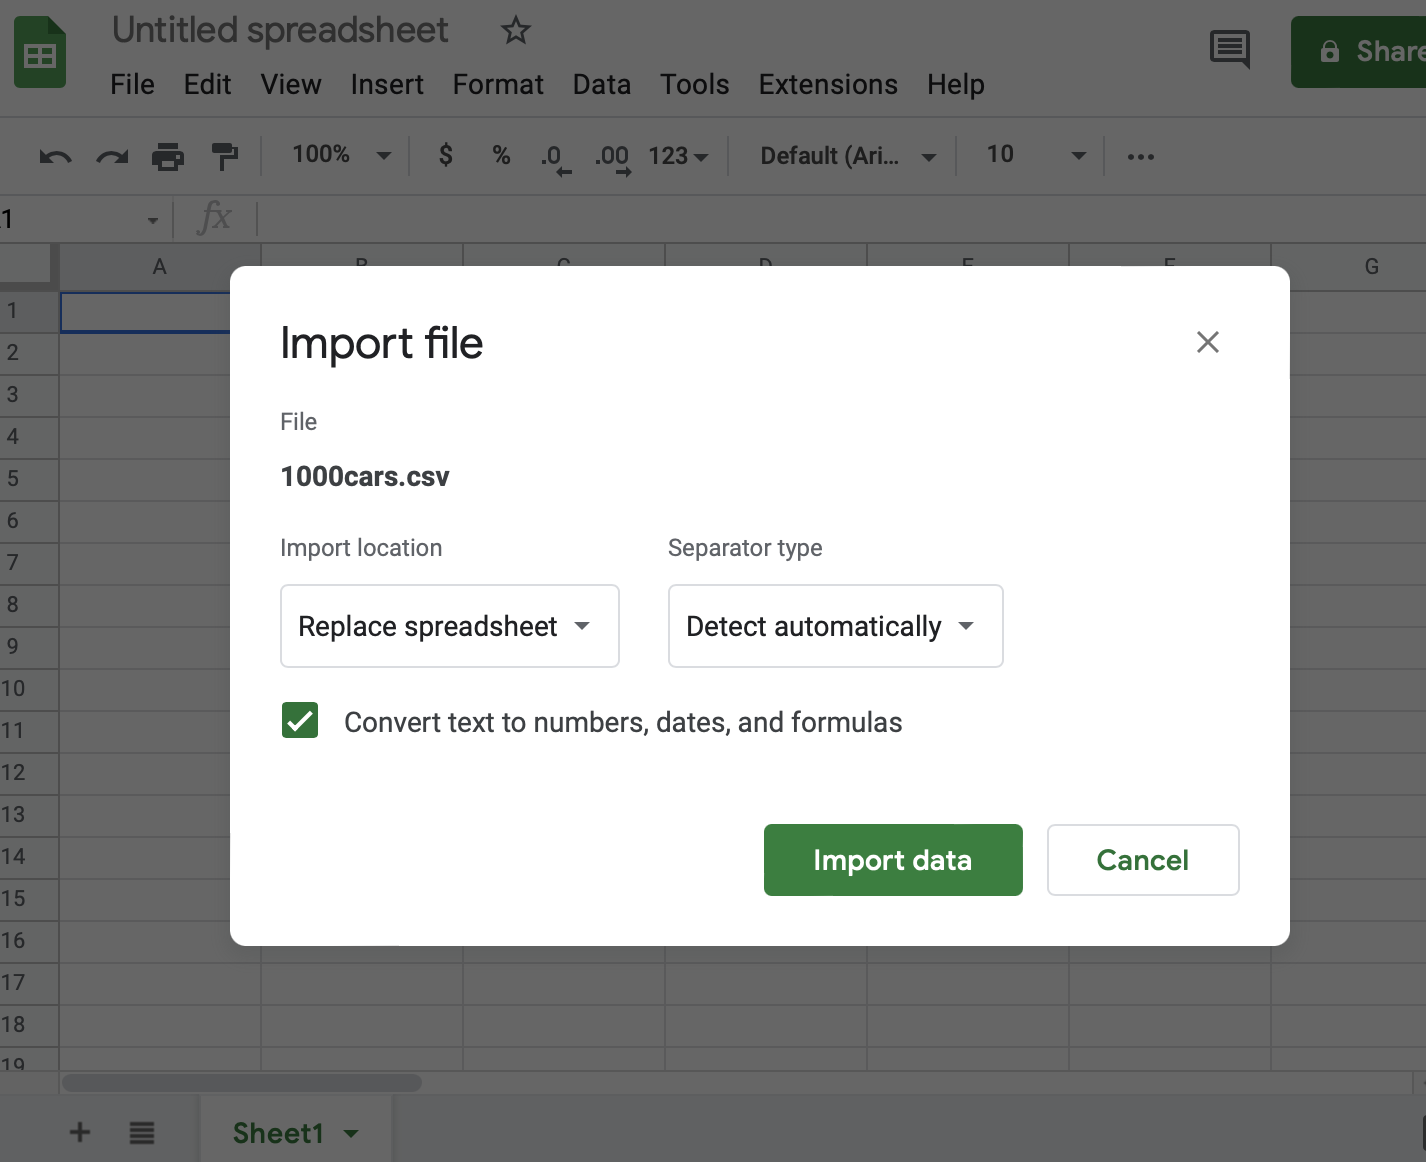
\includegraphics[width=0.5\textwidth]{ImportingCSV.png}

You should see a long, long column of data appear. (Mine goes from cell A2 through A1001.)

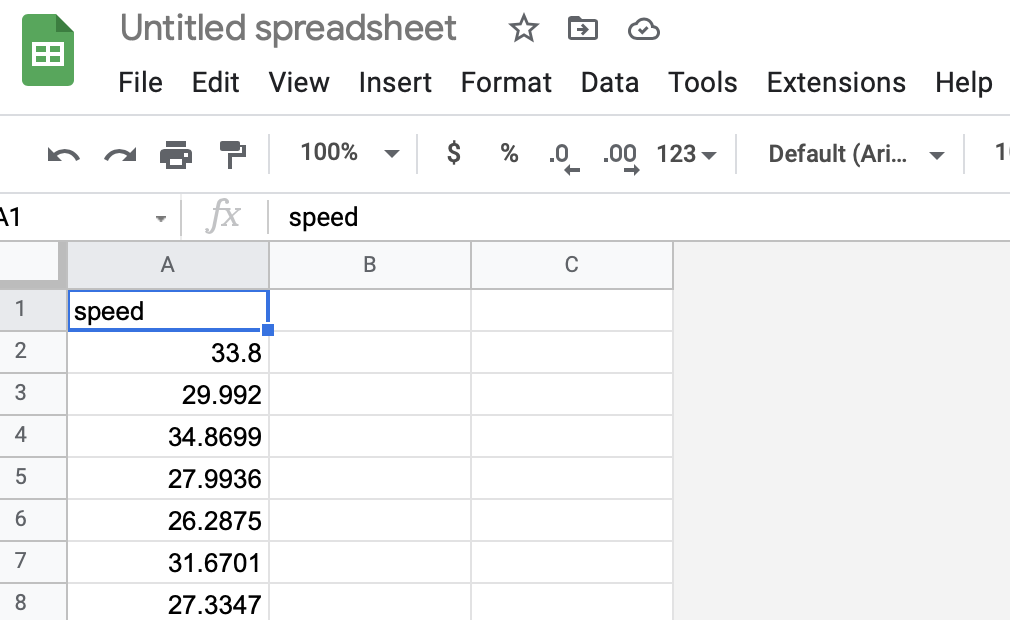
\includegraphics[width=0.5\textwidth]{ImportedCSV.png}

\subsection{Statistics in Spreadsheets}

Let us take the mean of all 1000 numbers.  In cell B2, type in a label:
``Mean''. (Feel free to format your labels as you wish. Bolding is recommended.)

In cell C2, enter the formula ``=AVERAGE(A2:A1001)''. When
you press return, the cell will show the mean: 31.70441, if done correctly.

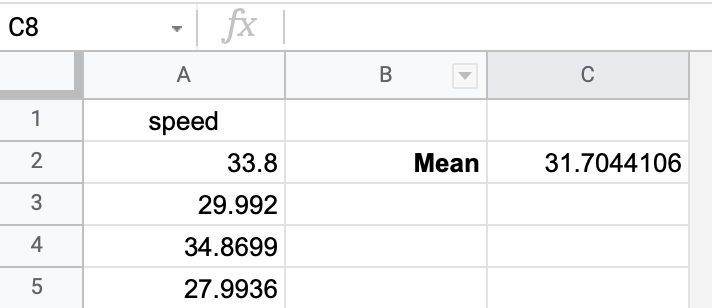
\includegraphics[width=0.4\textwidth]{Spread_mean.png}

Notice that by specifying that the function \pyfunction{AVERAGE} was to
be performed on a range of cells: cells A2 through (``:'') A1001.

Do the calculations for variance, standard deviation, and median.

\begin{itemize}
\item The function for variance is \pyfunction{VAR}.
\item The function for standard deviation is \pyfunction{STDEV}.
\item The function for median is \pyfunction{MEDIAN}.
\end{itemize}

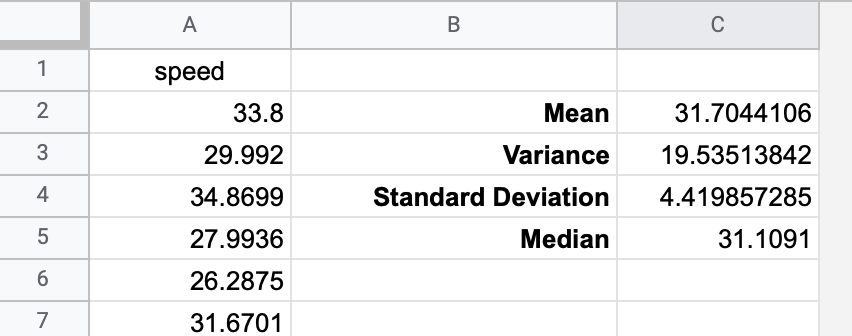
\includegraphics[width=0.4\textwidth]{var_stdev_median.png}

\subsection{Histogram}

Most spreadsheets have the ability to create a \index{histogram}histogram. In Google
Sheets, you select the entire range A2:A1001 by selecting the first
cell and then shift-clicking the last. Next, you choose
Insert$\rightarrow$Chart. In the inspector, change the type of the
chart to a histogram (at the bottom under ``other''). This will get you a basic histogram.
% Add: Define histogram or give example, defined in basic statistics, must come previous

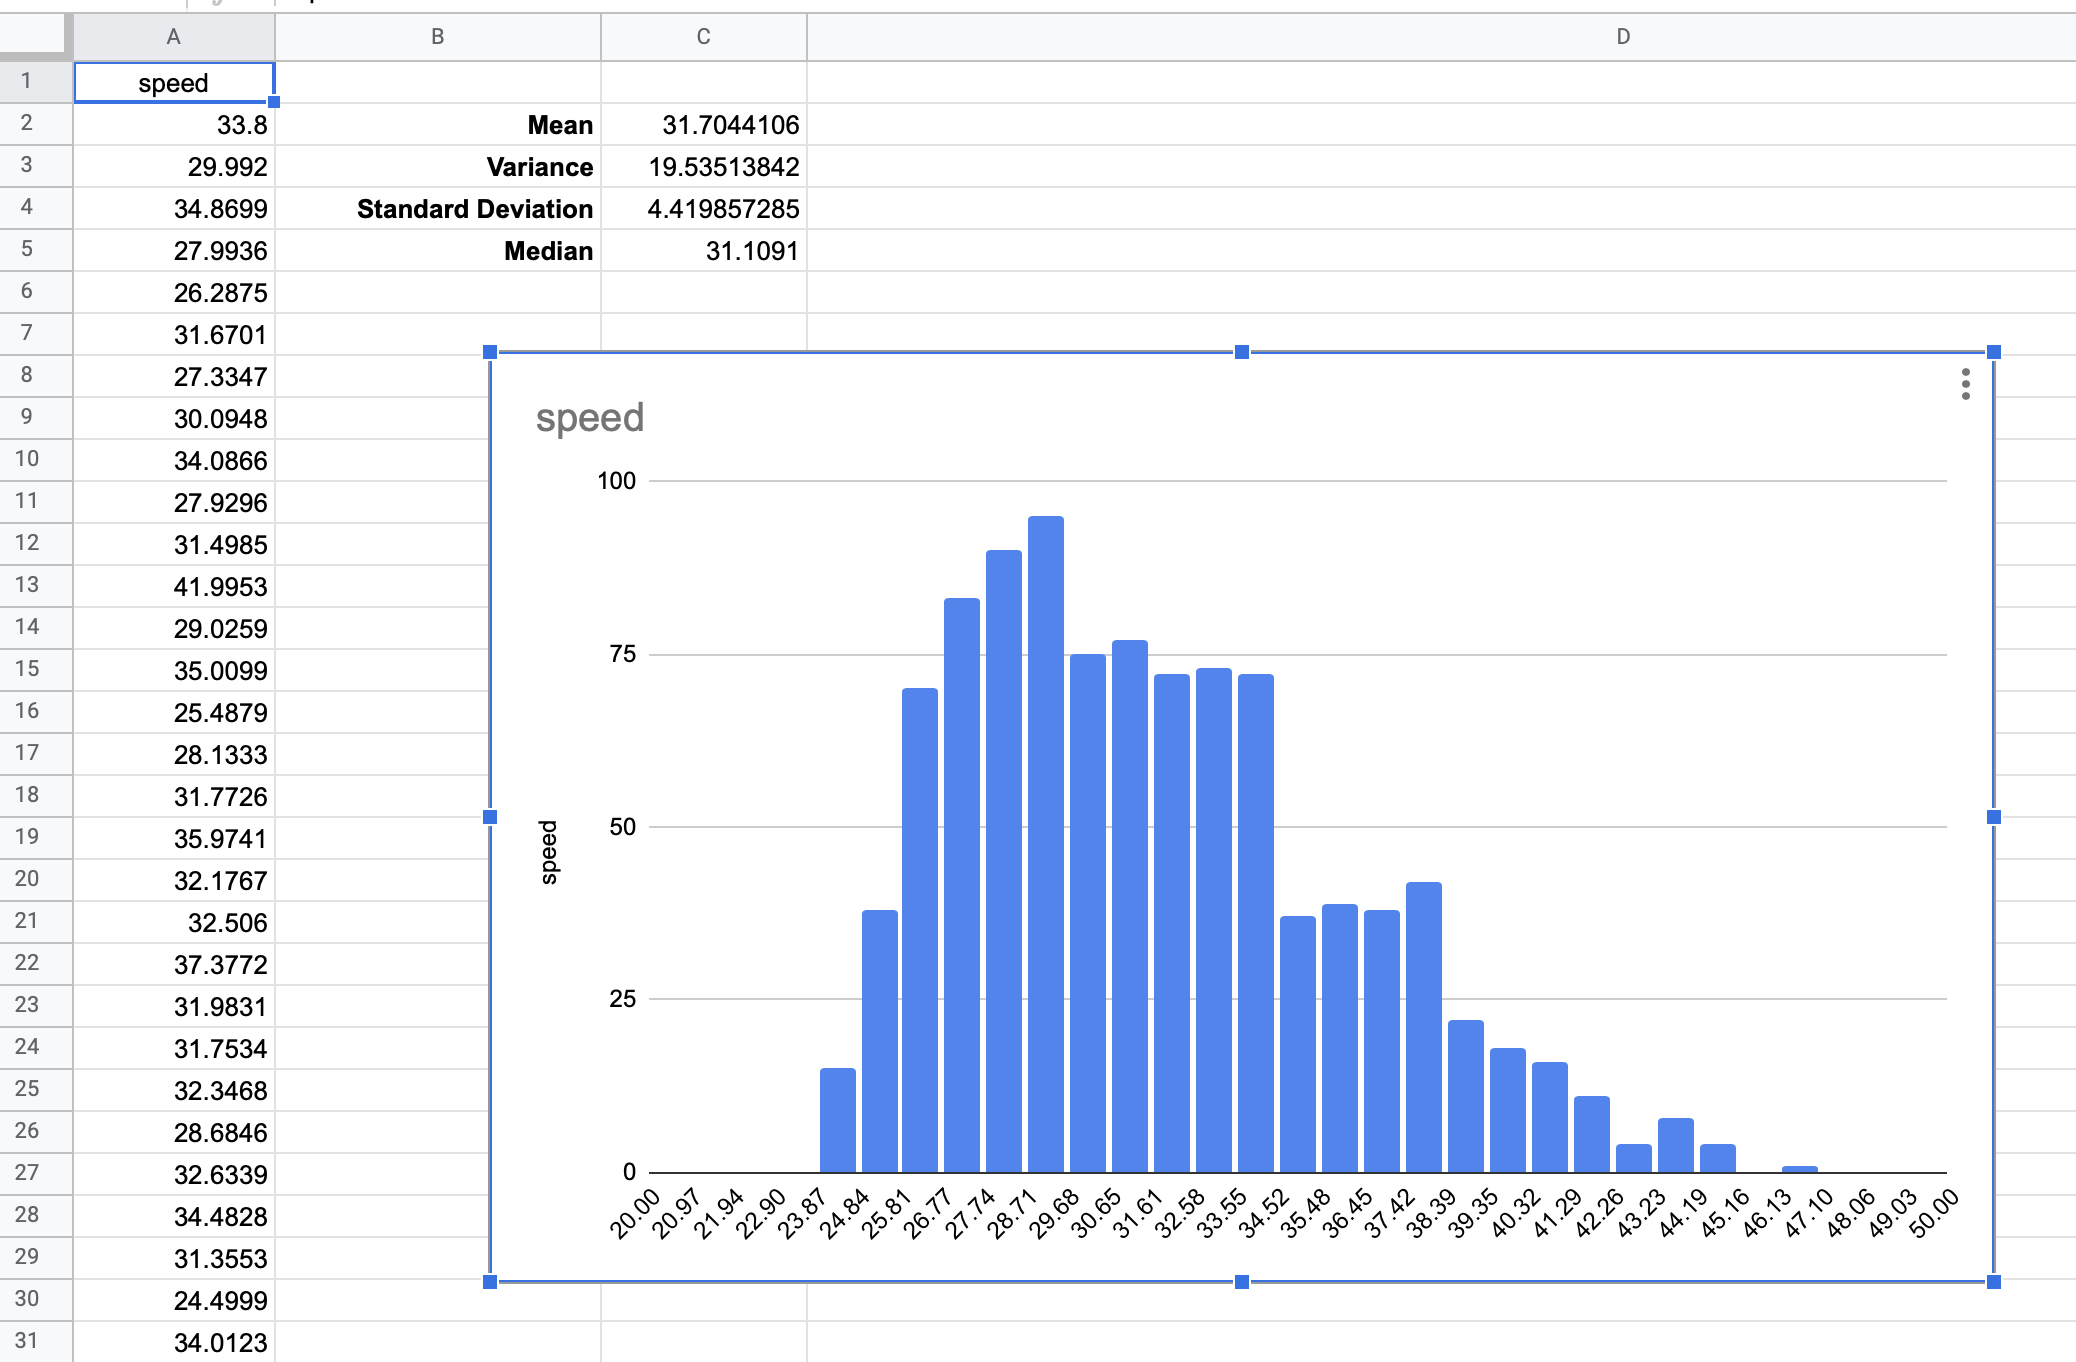
\includegraphics[width=0.7\textwidth]{default_histogram.png}

Play with the formatting to see how unique you can make data. Here is an example:

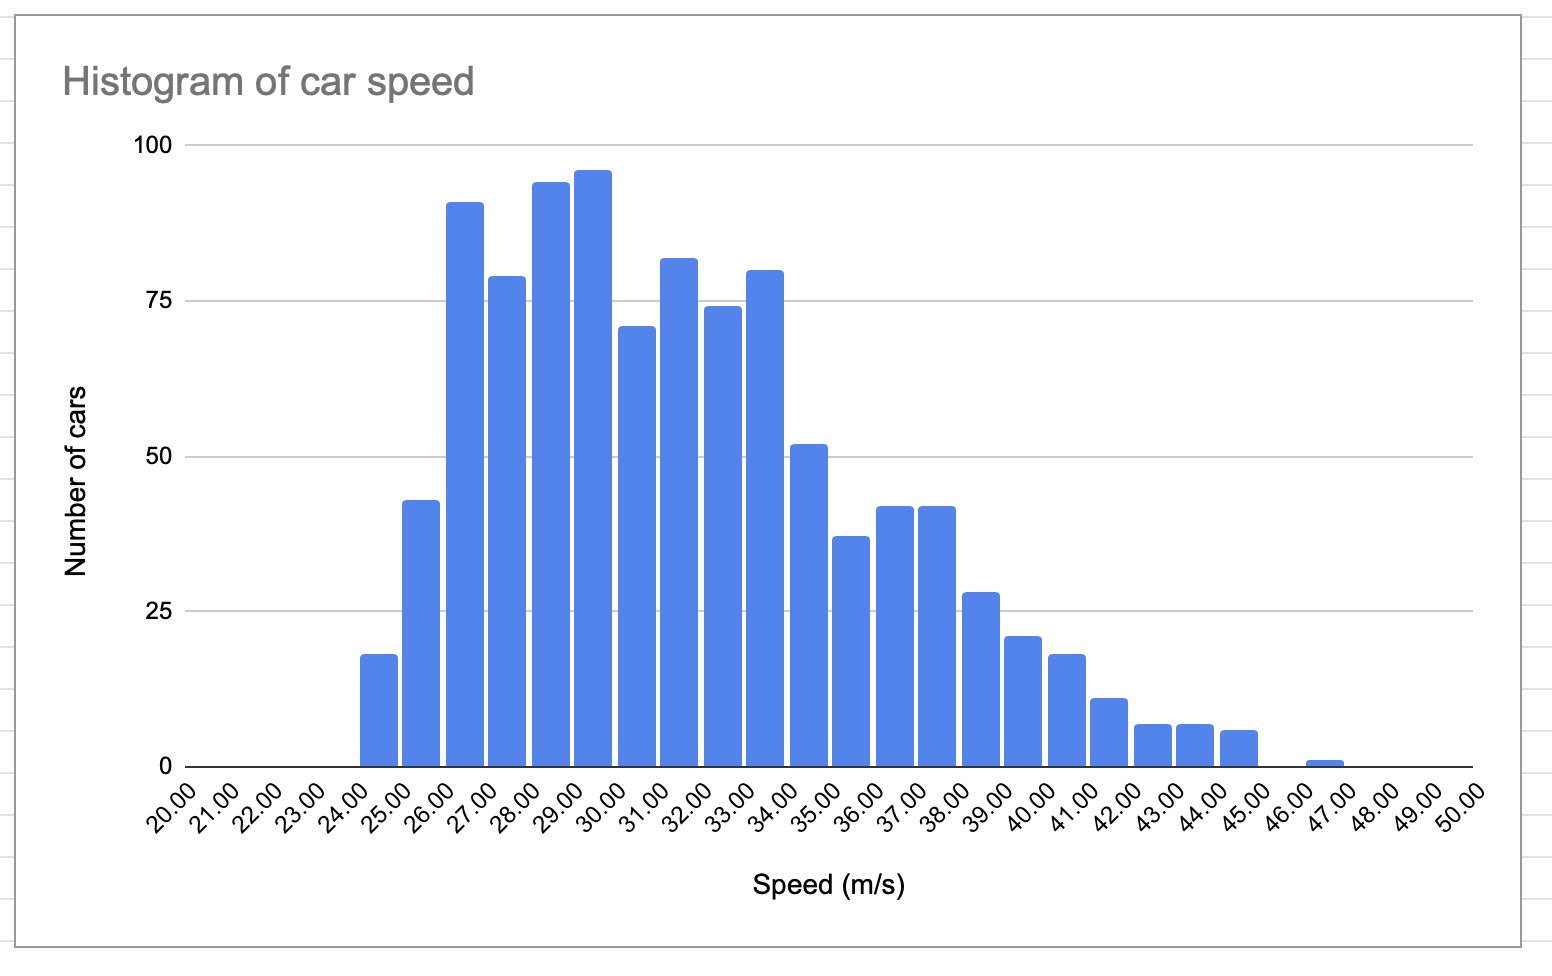
\includegraphics[width=0.8\textwidth]{final_histogram.png}

\begin{Exercise}[title={RMS}, label=rms_spreadsheet]

  In your spreadsheet, calculate the quadratic mean (the root-mean-squared\index{root-mean-squared}) of the speeds.

  You will need the following three functions:
  \begin{itemize}
  \item \pyfunction{SUMSQ} returns the sum of the squares of a range of cells.
  \item \pyfunction{COUNT} returns the number of cells in a range that contains numbers.
  \item \pyfunction{SQRT} returns the square root of a number.
  \end{itemize}


\end{Exercise}
\begin{Answer}[ref=rms_spreadsheet]

The formula for the RMS is ``=SQRT(SUMSQ(A2:A1001)/COUNT(A2:A1001))''.
% KA: https://www.khanacademy.org/computing/ap-computer-science-principles/data-analysis-101/data-tools/a/learning-from-data-sets

\end{Answer}


\subsection{The Return of the Barrel Problem}

Let us get back to our example. Put labels in the A column:
\begin{itemize}
\item{Barrels produced (per month)}
\item{Materials cost (per barrel)}
\item{Sale price (per barrel)}
\item{Pre-tax earnings (per month)}
\item{Taxes (per month)}
\item{Take home pay (per month)}
\end{itemize}

Format them any way you like. It should look something like this:

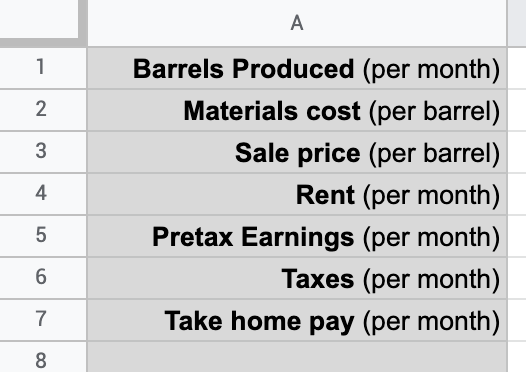
\includegraphics[width=0.4\textwidth]{BarrelLabels.png}

In the B column, the first four cells are values (not formulas):
\begin{itemize}
\item{115 formatted as a number with no decimal point}
\item{45 formatted as currency}
\item{100 formatted as currency}
\item{2000 formatted as currency}
\end{itemize}

It should look something like this:

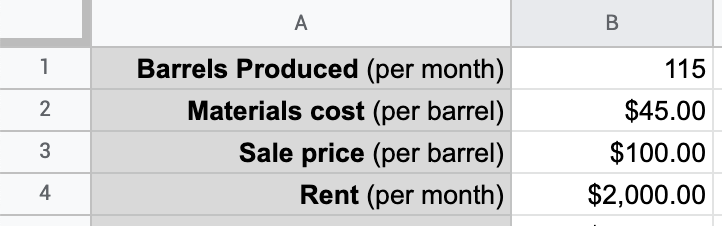
\includegraphics[width=0.5\textwidth]{BarrelValues.png}

The next three cells in the B column will have formulas:
\begin{itemize}
\item{B1 * (B3 - B2) - B4}
\item{0.2 * B5}
\item{B5 - B6}
\end{itemize}

It should look something like this:

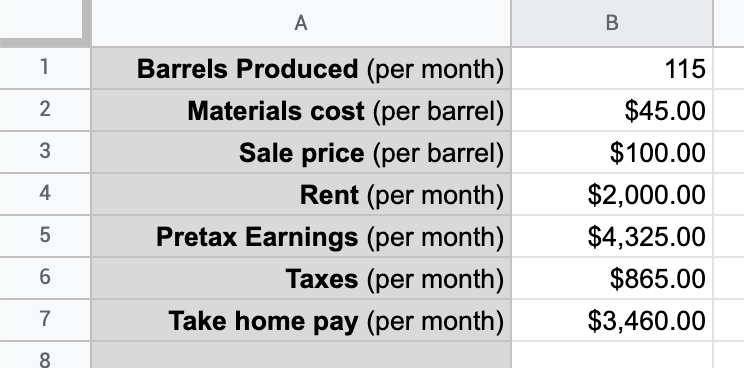
\includegraphics[width=0.5\textwidth]{BarrelFormulas.png}

Now you can share this spreadsheet with your friend, and she can put
different values into the cells for what-if games, such as ``If I can
get my materials cost down to \$42 per barrel, what happens to my take
home pay?''

Sometimes it is nice to show a range of values for a variable or two.
In this case, it might be nice to show your friend what the numbers
look like if she produces 115, 120, 125, 130, 135, or 140 barrels per
month.

We have one column, and now we need six. How do we duplicate cells?
\begin{enumerate}
\item Click B1 to select it, then shift-click on B7 to select all seven cells.
\item Copy them. (Depending on what program you are using, there is likely a menu item for this.)
\item Click C1 to select it
\item Paste them.
\end{enumerate}

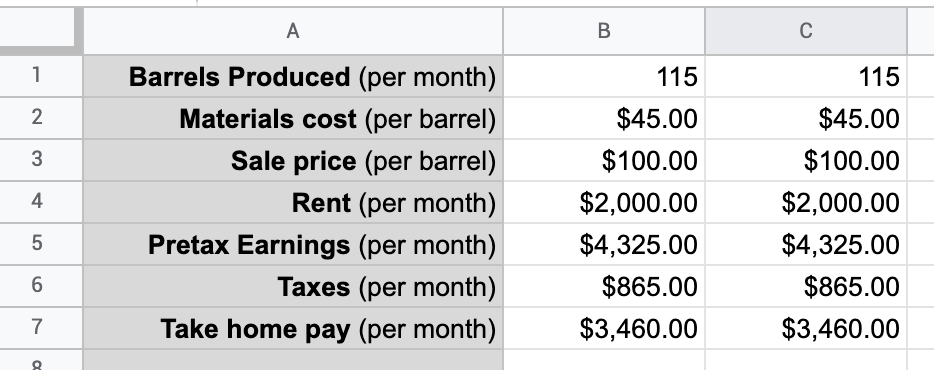
\includegraphics[width=0.5\textwidth]{BarrelCopyPaste.png}

We want the first cell in the new column to be 120. You could just
type in 120, but let us do something more clever. Put a formula into that
cell: = B1 + 5.  Now, the cell should show 120.

Why did we put in a formula? When we duplicate this column, this cell
will always have 5 more barrels than the cell to its left.

Next, let us duplicate the second column a few times. The easy way to do
this is to select the cells as you did before, then drag the lower-right
corner to the right until column G is in the selection. When you end
the drag, the copies will appear:

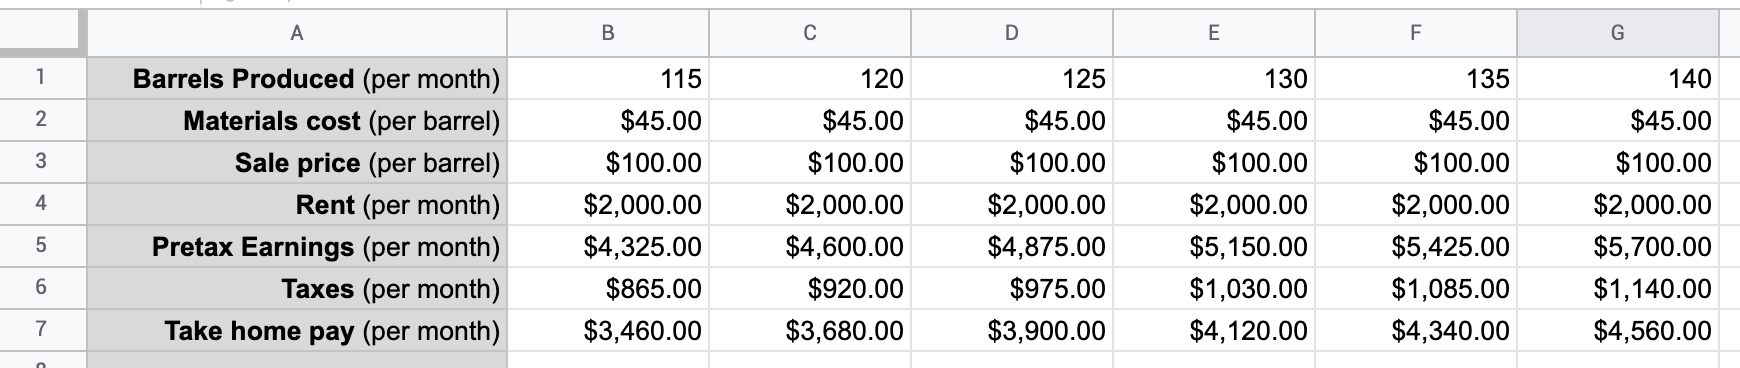
\includegraphics[width=0.8\textwidth]{BarrelDragPaste.png}

Nice, right? Now your friend can easily see how many barrels
correspond to how much take-home pay. But do you know what would be even more helpful? A graph.

\subsection{Graphing}

Graphing is a little different on every different platform.  Here is what you want the graph to look like:

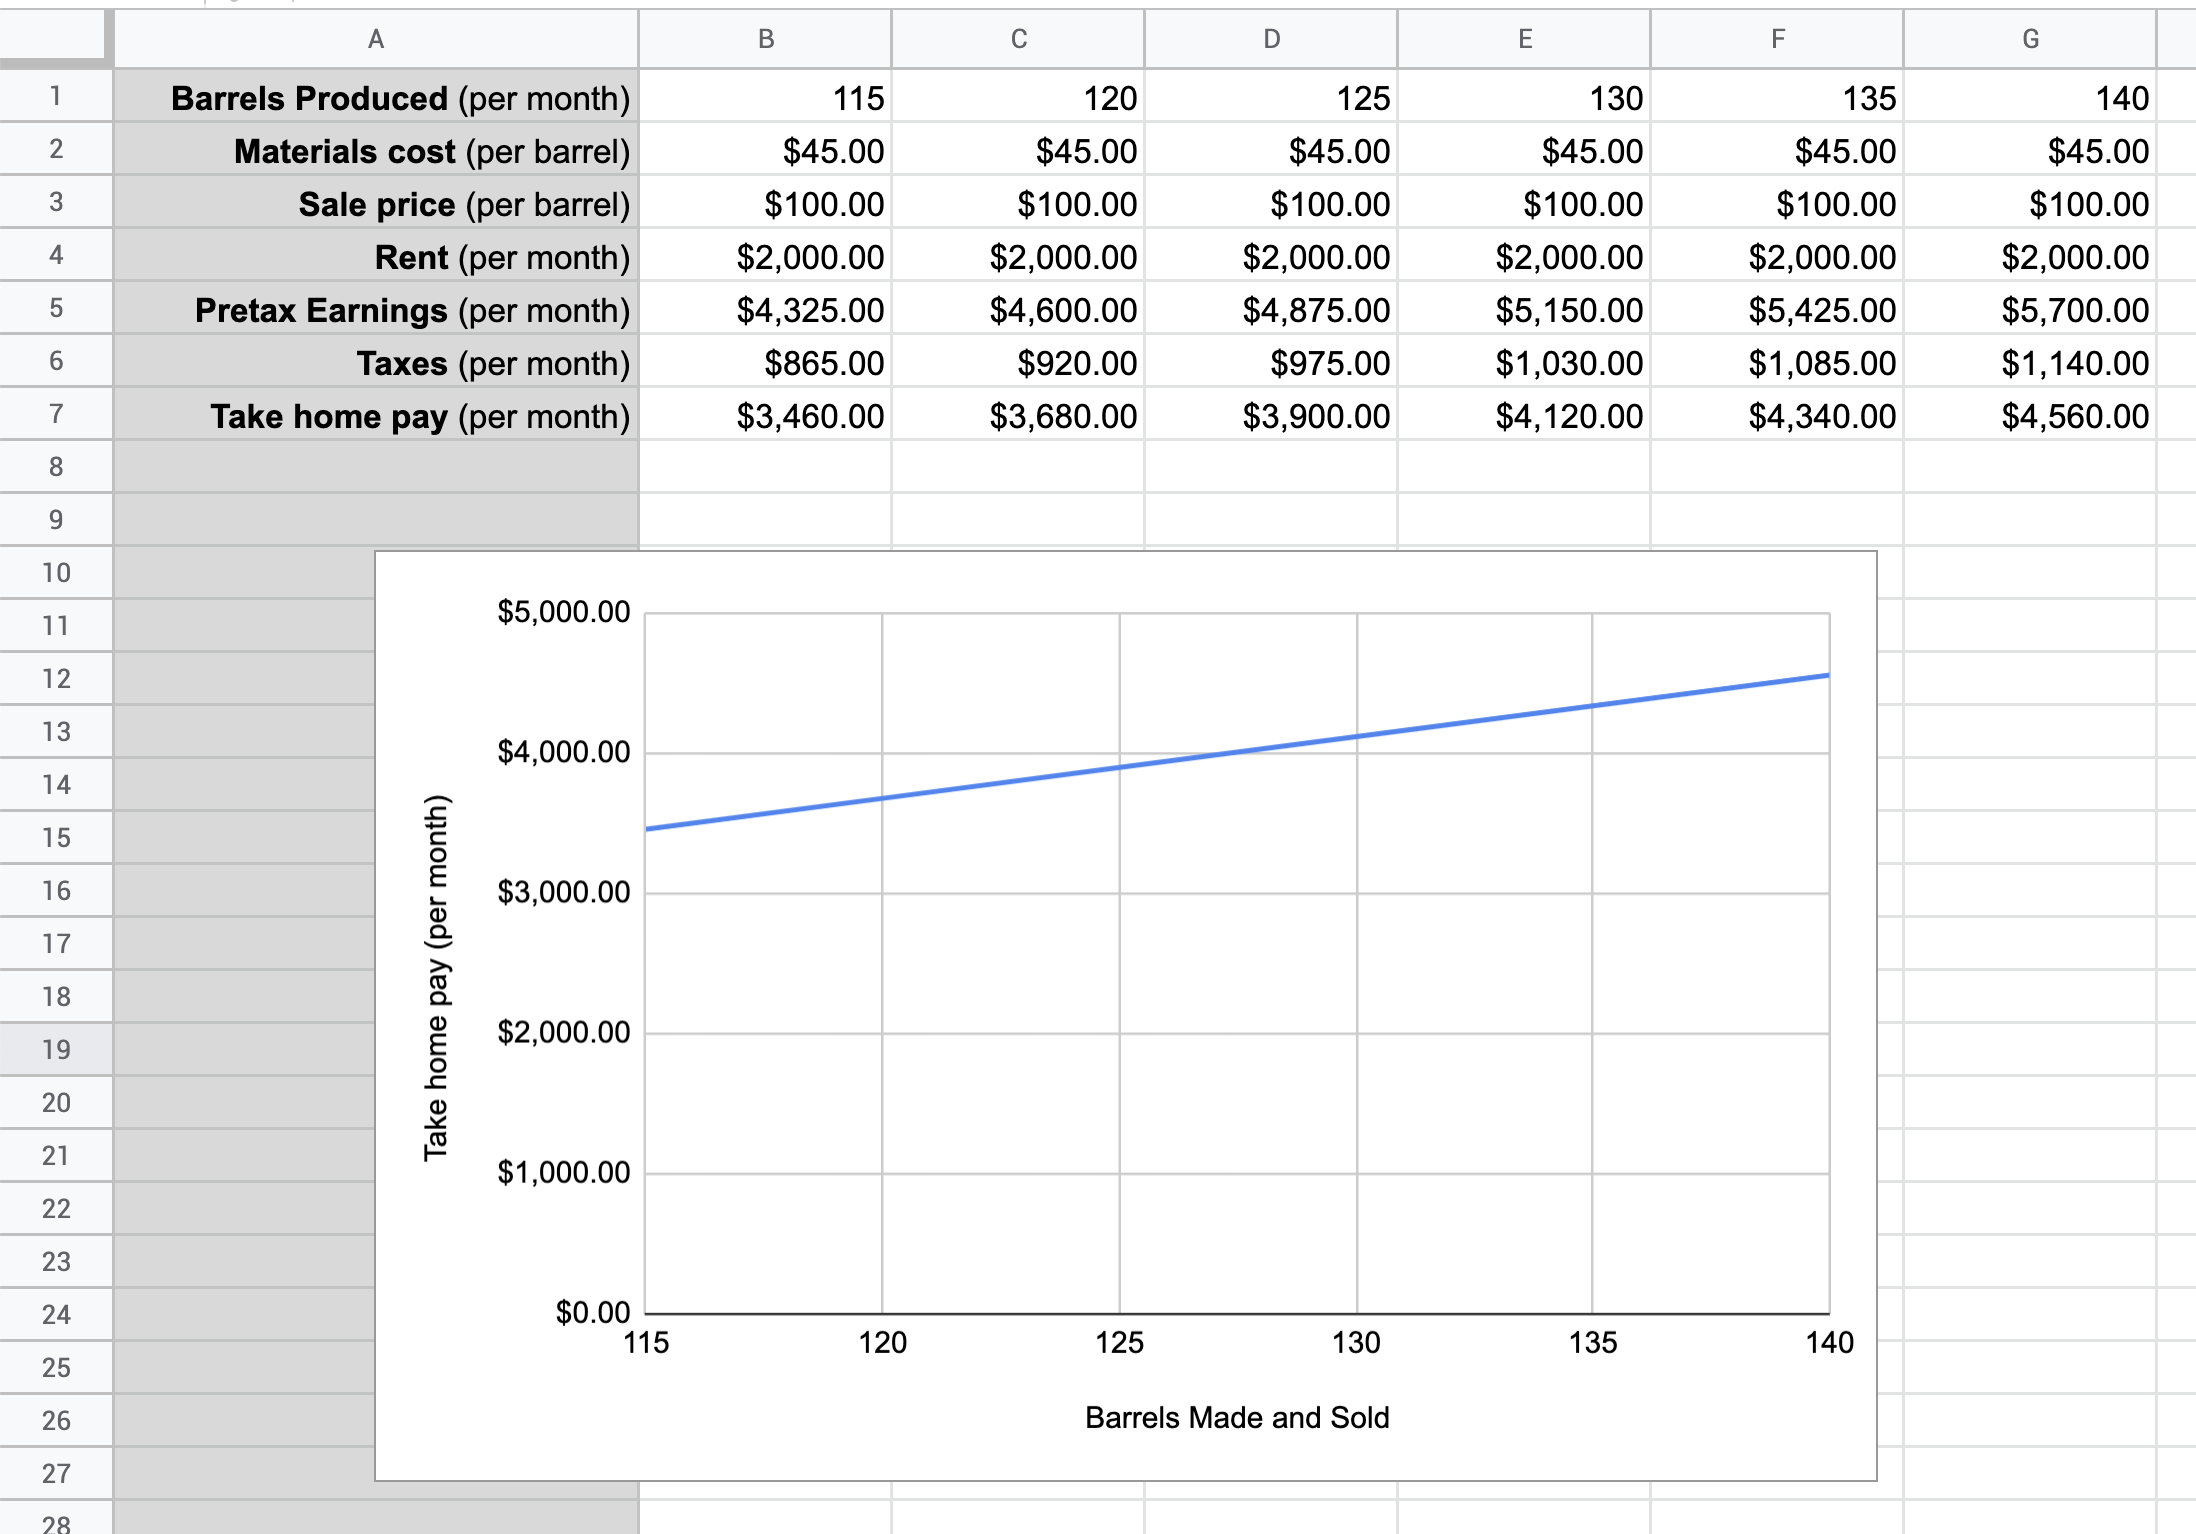
\includegraphics[width=0.8\textwidth]{BarrelGraph.png}

On Google Sheets:\index{spreadsheet!graphs}

\begin{enumerate}
\item Select cells B7 through G7. 
\item Choose the menu item Insert -> Chart.
\item Choose the chart type (Line)
\item Add the X-axis to be B1 through G1.
\item Under the Customize tab, Set the label for the X-axis to be ``Barrels Made and Sold''.
\item Delete the chart title (which is the same as the Y-axis label).
\end{enumerate}

\subsection{Other Things You Should Know About Spreadsheets}

Your spreadsheet document can have several ``Sheets''.  Each has its
own grid of cells.  The sheet has a name; usually, you call it
something like ``Salaries''.  When you need to use a value from the
``Salaries'' sheet in another sheet, you can specify ``Salaries!A2''
--- that is, cell A2 on sheet ``Salaries''.  To flip between the sheets,
there is usually a tab for each at the bottom of the document.

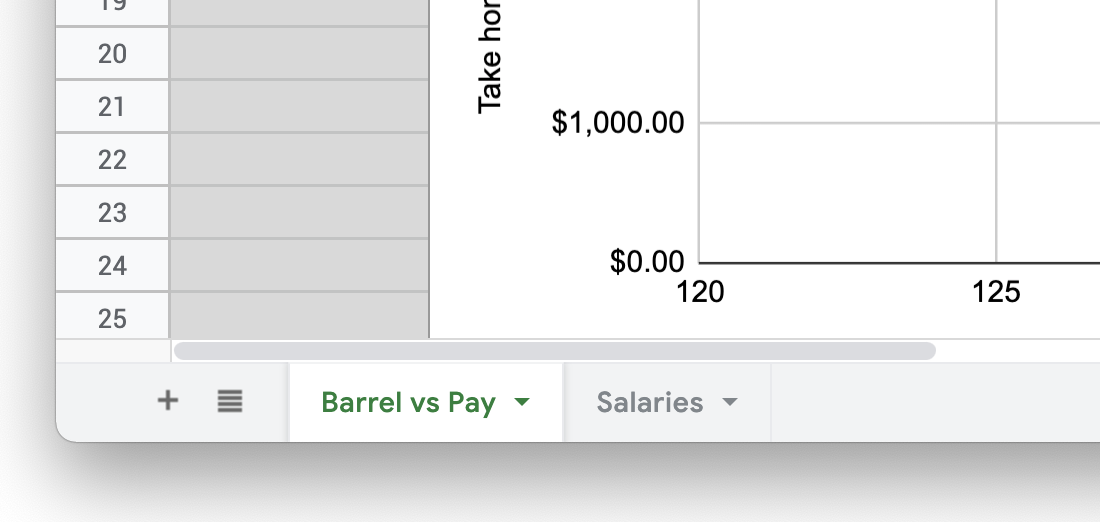
\includegraphics[width=0.5\textwidth]{Sheets.png}

By default, the cell references are \index{cell reference!relative}relative. In other words, when you write
a formula in cell H5 that references the value in cell G4, the cell
remembers ``The cell that is one up and one to the left of me.''
Thus, if you copy that formula into B9, now that formula reads the
value from A8.

If you want an \index{cell reference!absolute}absolute reference, you use \$. If H5 references
\$G\$4, G4 will be used no matter where on the sheet the formula is
copied to.

You can use the \$ on the row or column. In \$A4, the column is
absolute and the row is relative.  In A\$4, the row is absolute and
the column is relative.

\subsection{Challenge: Make a spreadsheet}

You have a company that bids on painting jobs. Make a
spreadsheet to help you do bids. Here are the parameters:
\begin{itemize}
\item The client will tell you how many square meters of wall needs to be painted.
\item Paint costs \$0.02 per square meter of wall
\item On average, a square meter of wall takes 0.02 hours to paint.
\item You can hire painters at \$15 per hour.
\item You add 20\% to your estimated costs for a margin of error and profit.
\end{itemize}

Make a spreadsheet such that when you type in the square meters to be
painted, the spreadsheet tells you how much you will spend on paint
and labor.  It should also tell you what your bid should be.


\section{Data Analysis with jamovi}
A student club surveyed 100 classmates about sleep, screen time, breakfast, and a short quiz. The club wants to know what the answers show. This chapter introduces Jamovi, which is a free software that does the data analysis calculations for you.

\subsection{Getting Started with jamovi}

\newterm{jamovi}\index{jamovi} is a free statistics program. You choose an analysis from a menu, tick a few boxes, and the results appear right away.

You can use jamovi in two ways:
\begin{itemize}
    \item In a web browser, at \url{https://cloud.jamovi.org}, with a free Guest account. Nothing needs to be installed.
    \item On your own computer, by downloading it from \url{https://www.jamovi.org}. This version works without the internet.
\end{itemize}

The jamovi window has three parts:
\begin{itemize}
    \item On the left, the \newterm{spreadsheet}\index{spreadsheet} holds the data. Each row is one person or thing, and each column is one variable.
    \item Across the top, the \newterm{analysis ribbon}\index{analysis ribbon} lists the analyses you can run.
    \item The \newterm{results panel}\index{results panel} on the right shows tables and graphs.
\end{itemize}

% [figure placeholder: jamovi window with the three parts labeled]

To try it, open an example dataset. Click the menu icon (three lines) in the top-left corner, then choose Open, Data Library, Examples, and Tooth Growth. On the Analyses tab, click Exploration, then Descriptives, and move \texttt{len} into the Variables box. A table of statistics appears without pressing any Run button.

% [C: confirm this menu path in the current jamovi Cloud interface before publication]

\begin{Exercise}[title={Which Part of the Window?}, label={ex:jamovi-regions}]
Name the part of the window you would use for each task: spreadsheet, analysis ribbon, or results panel.

\begin{center}
\begin{tabular}{|p{8cm}|p{4cm}|}
\hline
Task & Part \\
\hline
Fix a number that was typed wrong & \\
\hline
Choose an analysis & \\
\hline
Read the mean & \\
\hline
\end{tabular}
\end{center}
\end{Exercise}
\begin{Answer}[ref={ex:jamovi-regions}]
\begin{center}
\begin{tabular}{|p{8cm}|p{4cm}|}
\hline
Task & Part \\
\hline
Fix a number that was typed wrong & Spreadsheet \\
\hline
Choose an analysis & Analysis ribbon \\
\hline
Read the mean & Results panel \\
\hline
\end{tabular}
\end{center}
\end{Answer}

\subsection{Setting Up Your Data}

Find \texttt{student\_survey.csv} in your digital resources. Click the menu icon, choose Open, then Browse, and select the file. In jamovi Cloud, you may need to upload it first.

% [C: confirm the Cloud upload and open steps in the current interface ]

\begin{center}
\begin{tabular}{|l|p{9cm}|}
\hline
Column & What it records \\
\hline
\texttt{student\_id} & A code number for each student \\
\hline
\texttt{travel} & How the student gets to school: Walk, Cycle, Bus, or Car \\
\hline
\texttt{breakfast} & Whether the student ate breakfast: Yes or No \\
\hline
\texttt{screen\_time} & Hours on screens per day \\
\hline
\texttt{sleep\_hours} & Hours of sleep per night \\
\hline
\texttt{sleep\_quality} & The student's sleep rating: Poor, Fair, or Good \\
\hline
\texttt{quiz\_score} & Score on a 20-point quiz \\
\hline
\end{tabular}
\end{center}

jamovi gives each column a \newterm{measure type}\index{measure type}, which tells it what kind of data the column holds:
\begin{itemize}
    \item Nominal: categories with no order, such as travel method
    \item Ordinal: categories with an order, such as Poor, Fair, Good
    \item Continuous: measured numbers, such as hours of sleep
    \item ID: labels for each case, such as a student code
\end{itemize}

jamovi guesses these types when it opens a file, and it can guess wrong. To fix one, double-click the column name and pick the correct type.

Two cells in \texttt{sleep\_hours} are empty because those students skipped the question. jamovi treats empty cells as \newterm{missing values}\index{missing values} and leaves them out of calculations.

\begin{Exercise}[title={Measure Types}, label={ex:jamovi-measure-types}]
Give the correct measure type for each column.

\begin{center}
\begin{tabular}{|l|p{4cm}|}
\hline
Column & Measure type \\
\hline
\texttt{student\_id} & \\
\hline
\texttt{breakfast} & \\
\hline
\texttt{sleep\_hours} & \\
\hline
\texttt{sleep\_quality} & \\
\hline
\end{tabular}
\end{center}
\end{Exercise}
\begin{Answer}[ref={ex:jamovi-measure-types}]
\begin{center}
\begin{tabular}{|l|p{4cm}|}
\hline
Column & Measure type \\
\hline
\texttt{student\_id} & ID \\
\hline
\texttt{breakfast} & Nominal \\
\hline
\texttt{sleep\_hours} & Continuous \\
\hline
\texttt{sleep\_quality} & Ordinal \\
\hline
\end{tabular}
\end{center}
\end{Answer}

\subsection{Describing Data}

\index{descriptive statistics}Click Exploration, then Descriptives. Move \texttt{quiz\_score} and \texttt{sleep\_hours} into the Variables box.

\begin{center}
\begin{tabular}{|l|r|r|}
\hline
 & \texttt{quiz\_score} & \texttt{sleep\_hours} \\
\hline
N & 100 & 98 \\
\hline
Missing & 0 & 2 \\
\hline
Mean & 12.40 & 7.51 \\
\hline
Median & 12 & 7.60 \\
\hline
Standard deviation & 3.35 & 0.99 \\
\hline
Minimum & 4 & 4.5 \\
\hline
Maximum & 20 & 9.8 \\
\hline
\end{tabular}
\end{center}

The average quiz score was 12.4 out of 20. Students slept 7.51 hours a night on average.

To compare groups, move a category into the Split by box. To draw a graph, open Plots and tick Histogram or Box plot. For a category such as \texttt{travel}, tick Frequency tables to count how many students are in each group.

% [figure placeholder: box plots of quiz_score split by breakfast]

\begin{Exercise}[title={Breakfast and Quiz Scores}, label={ex:jamovi-split}]
Put \texttt{quiz\_score} in the Variables box and \texttt{breakfast} in the Split by box.
\begin{enumerate}
\item What is the median quiz score for each group?
\item Which group did better?
\end{enumerate}
\end{Exercise}
\begin{Answer}[ref={ex:jamovi-split}]
\begin{enumerate}
\item Breakfast: 13 points. No breakfast: 11 points.
\item Students who ate breakfast had the higher median score.
\end{enumerate}
\end{Answer}

\subsection{Comparing Two Groups}

Students who ate breakfast averaged 13.28 on the quiz, and students who skipped it averaged 11.03. A t-test checks whether a gap this large could be due to chance.

\index{t-test}Click T-Tests, then Independent Samples T-Test. Move \texttt{quiz\_score} into Dependent Variables and \texttt{breakfast} into Grouping Variable. Under Tests, tick \index{Welch's t-test}Welch's and untick Student's. Welch's version is the safer choice because it does not require the two groups to have the same spread.

% [figure placeholder: t-test options panel with Welch's ticked]

jamovi reports $t = -3.40$ and $p = 0.001$. A small $p$-value, below 0.05, means the gap is unlikely to be due to chance alone.

The negative sign appears because jamovi subtracts the Yes group from the No group. The breakfast group still scored higher.

These data come from a survey, so they show a link between breakfast and quiz scores. They cannot show that breakfast causes higher scores.

\begin{Exercise}[title={Reading the t-Test}, label={ex:jamovi-ttest}]
\begin{enumerate}
\item Is $p = 0.001$ below 0.05?
\item Write one sentence explaining what the test shows.
\end{enumerate}
\end{Exercise}
\begin{Answer}[ref={ex:jamovi-ttest}]
\begin{enumerate}
\item Yes.
\item Students who ate breakfast scored higher on the quiz, and the difference is too large to blame on chance alone.
\end{enumerate}
\end{Answer}

\subsection{Looking at Relationships}

Does more screen time go with less sleep? Click Exploration, then Scatterplot. Put \texttt{screen\_time} on the X-Axis and \texttt{sleep\_hours} on the Y-Axis.
% [C: confirm the Scatterplot item appears under Exploration in the current Cloud version]

% [figure placeholder: scatterplot of sleep_hours against screen_time]

The points slope downward: more screen time goes with less sleep.

Click Regression, then Correlation Matrix, and add both variables. The \newterm{correlation}\index{correlation} $r$ runs from $-1$ to $1$ and measures how closely the points follow a straight line. Here $r = -0.70$, a strong negative relationship.

For a line of best fit, open Regression, then Linear Regression. Put \texttt{sleep\_hours} in Dependent Variable and \texttt{screen\_time} in Covariates. jamovi gives the line
\[
\widehat{\text{sleep}} = 9.55 - 0.44 \times \text{screen time}
\]
Each extra hour of screen time goes with about 0.44 fewer hours of sleep.

\begin{Exercise}[title={Making a Prediction}, label={ex:jamovi-predict}]
Use the line to predict the sleep of a student with 6 hours of screen time.
\end{Exercise}
\begin{Answer}[ref={ex:jamovi-predict}]
$9.55 - 0.44 \times 6 = 6.91$ hours of sleep.
\end{Answer}

\subsection{Saving Your Work}

Click the menu icon and choose Save As. jamovi saves an \newterm{.omv file}\index{.omv file}, which keeps your data and results together. In jamovi Cloud, download a copy to your own device before closing the tab.
% [C: confirm current Guest plan file-retention behavior in jamovi Cloud before publication]

To put a table or graph in a report, right-click it and choose Copy, then paste it into your document.

\begin{Exercise}[title={Saving Choices}, label={ex:jamovi-saving}]
\begin{enumerate}
\item Which file type keeps both your data and your results?
\item How do you move a table into a report?
\end{enumerate}
\end{Exercise}
\begin{Answer}[ref={ex:jamovi-saving}]
\begin{enumerate}
\item An .omv file.
\item Right-click the table, choose Copy, and paste it into the report.
\end{enumerate}
\end{Answer}


With jamovi you can open data, set it up, describe it, test it, and save your results, all without writing code. Because it is free and runs in a browser, you can use it on almost any device.
